\documentclass[a4paper,titlepage]{article}
\title{CT Projekt: Raycasting engine (Hundefels 2D)}
\author{Christian Korn}
\date{20.10.2021 - 11.01.2022}

\usepackage[ngerman]{babel}
\usepackage{graphicx}

\begin{document}
\maketitle
\tableofcontents

\newpage

\section{Ziele}

\subsection{Muss-Ziele}
Wenn diese Ziele nicht erreicht werden, wird das Projekt als Fehlschlag angesehen.

\begin{itemize}
\item Anzeigen eines 2D Levels in 2,5D (Raycasting Methode)
\item Bewegungsfreiheit im Level (Translation und Rotation)
\end{itemize}

\subsection{Soll-Ziele}
Diese Ziele müssen nicht unbedingt erreicht werden, sind aber für einen vollen Erfolg nötig.

\begin{itemize}
\item Laden von Leveln aus Dateien
\item Anzeigen von anderen Objekten im Level (z.B. Gegner, Items)
\item Kollisionserkennung
\end{itemize}

\subsection{Kann-Ziele}
Diese Ziele sind nicht nötig, können aber nach Vollendung der Höheren Ziele in Angriff genommen werden.

\begin{itemize}
\item Gegner KI
\item Schießen
\item Sprites
\item Texturen für Wände
\item visuelle Effekte (view bobbing, Blutspritzer)
\end{itemize}

\newpage

\section{Verwendete Technologien}

\subsection{Python}

Das Projekt wurde mit Python \verb|3.9.7| erstellt, müsste aber auch in späteren Versionen funktionieren.

\subsubsection*{Externe Libraries}

\begin{itemize}
	\item Pygame: Installation mit ``\verb|pip install pygame|''
	Verwendet für Darstellung.
	\item Numba: Installation mit ``\verb|pip install numba|''
	Für `magische' Leistungsverbesserungen von besonders aufwändigen Funktionen durch JIT-Compilierung.
\end{itemize}

\subsubsection*{IDE}

Es wurde die PyCharm Community Edition verwendet.

\subsection{Dokumentation}

Die Projektdokumentation wurde mit \LaTeX erstellt,
UML Klassendiagramme wurden mit YUML erstellt.

\subsection{Versionskontrollsystem}

Ein GIT Repository wurde angelegt. Es kann unter \verb|https://github.com/MacAphon/hundefels2d| gefunden werden.

\newpage
\section{Mathematische Funktionsweise}

Die Berechnungen werden 1 mal pro Frame ausgeführt. Idealerweise heißt das, dass sie 60 mal pro Sekunde erfolgen. wenn die Rechenleistung nicht ausreicht wird eine Warnung angezeigt.

\subsection{Bewegung}

Der aktuelle Bewegungszustand und die Position werden in den Variablen \verb|_state| und \verb|_position| gespeichert.

\subsubsection*{Drehung}

Solange $\leftarrow$ oder $\rightarrow$ gedrückt werden wird der


\subsubsection*{Laufen}

\subsection{Darstellung}
\setlength{\unitlength}{1cm}
Horizontaler Check
\\
\begin{picture}(5,4)
	% Gitternetz
	\multiput(0,0)(1,0){6}{\line(0,1){4}}
	\linethickness{0.4mm}
	\multiput(0,0)(0,1){5}{\line(1,0){5}}
	\thinlines
	% Wand
	\multiput(0,0)(0.1,0){50}{\line(0,1){1}}
	% Spieler und Sichtlinie
	\put(1,3){\circle*{0.3}}
	\thicklines
	\put(1,3){\vector(4,-3){2.7}}
	% Kreuzpunkte
	\linethickness{0.6mm}
	\put(2.35,1.75){\line(0,1){0.5}}
	\put(2.1,2){\line(1,0){0.5}}
	\put(3.68,0.75){\line(0,1){0.5}}
	\put(3.43,1){\line(1,0){0.5}}
\end{picture}
\\
Vertikaler Check
\\
\begin{picture}(5,4)
	% Gitternetz
	\linethickness{0.4mm}
	\multiput(0,0)(1,0){6}{\line(0,1){4}}
	\thinlines
	\multiput(0,0)(0,1){5}{\line(1,0){5}}
	% Wand
	\multiput(0,0)(0.1,0){50}{\line(0,1){1}}
	% Spieler und Sichtlinie
	\put(1,3){\circle*{0.3}}
	\thicklines
	\put(1,3){\vector(4,-3){3}}
	% Kreuzpunkte
	\linethickness{0.6mm}
	\put(2,2){\line(0,1){0.5}}
	\put(1.75,2.25){\line(1,0){0.5}}
	\put(3,1.25){\line(0,1){0.5}}
	\put(2.75,1.5){\line(1,0){0.5}}
	\put(4,0.5){\line(0,1){0.5}}
	\put(3.75,0.75){\line(1,0){0.5}}
\end{picture}

\newpage

\section{Programmaufbau}
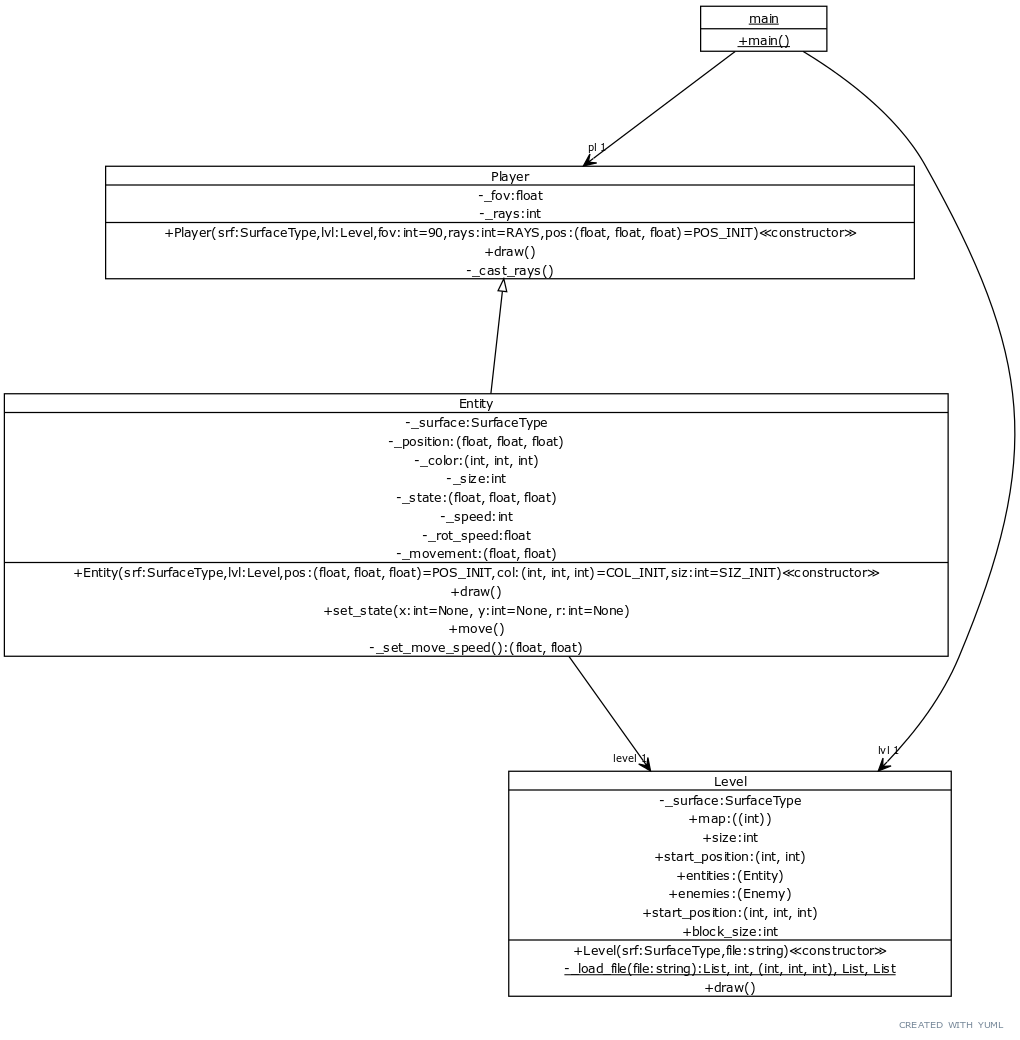
\includegraphics[scale=0.35]{./img/yuml1}

\newpage

\section{Steuerung}

\subsection{Command-Line Argumente}

\begin{itemize}
	\item \verb|-h --help| zeigt die CLI Argumente und beendet das Programm.
	\item \verb|-l --level| lädt das angegebene Level oder die angegebene Level Datei.
	\item \verb|--fov| ändert den Blickwinkel (angegeben in Grad) Standartwert ist 90°.
	\item \verb|--rays| ändert die horizontale Auflösung (Anzahl der gesendeten Strahlen) Standartwert ist 90. Höhere Werte können die Leistung beeinträchtigen.
\end{itemize}

\subsection{Levelerstellung}
Level werden im JSON-Format gespeichert.
\begin{itemize}
	\item \verb|"map": [[int]]| Die Map: 1 entspricht einer Wand, 0 Leerraum. Die Map muss quadratisch sein (ansonsten crasht das Programm)
	\item \verb|"size": int| Die Größe der Map. Muss dem tatsächlichen Wert entsprechen.
	\item \verb|"start_pos": [x: int, y: int, r: int]| Die Startposition des Spielers. \verb|x| und \verb|y| sind Werte zwischen 0 und 512, sie geben die Position in Pixeln an. \verb|r| ist zwischen 0 und 360 und ist die Drehung in Grad.
	\item \verb|"entities": [], "enemies": []| Enthalten aktuell keine Werte und werden für zukünftigen Gebrauch freigehalten.
	
\end{itemize}

\subsection{Bewegung}

\subsubsection*{Translation (Laufen)}
\begin{itemize}
\item Vorwärts: `W'
\item Links: `A'
\item Rückwärts: `S'
\item Rechts: `D'
\end{itemize}

\subsubsection*{Rotation}
\begin{itemize}
\item Links: linke Pfeiltaste ($\leftarrow$)
\item Rechts: rechte Pfeiltaste ($\rightarrow$)
\end{itemize}

\subsection{UI}
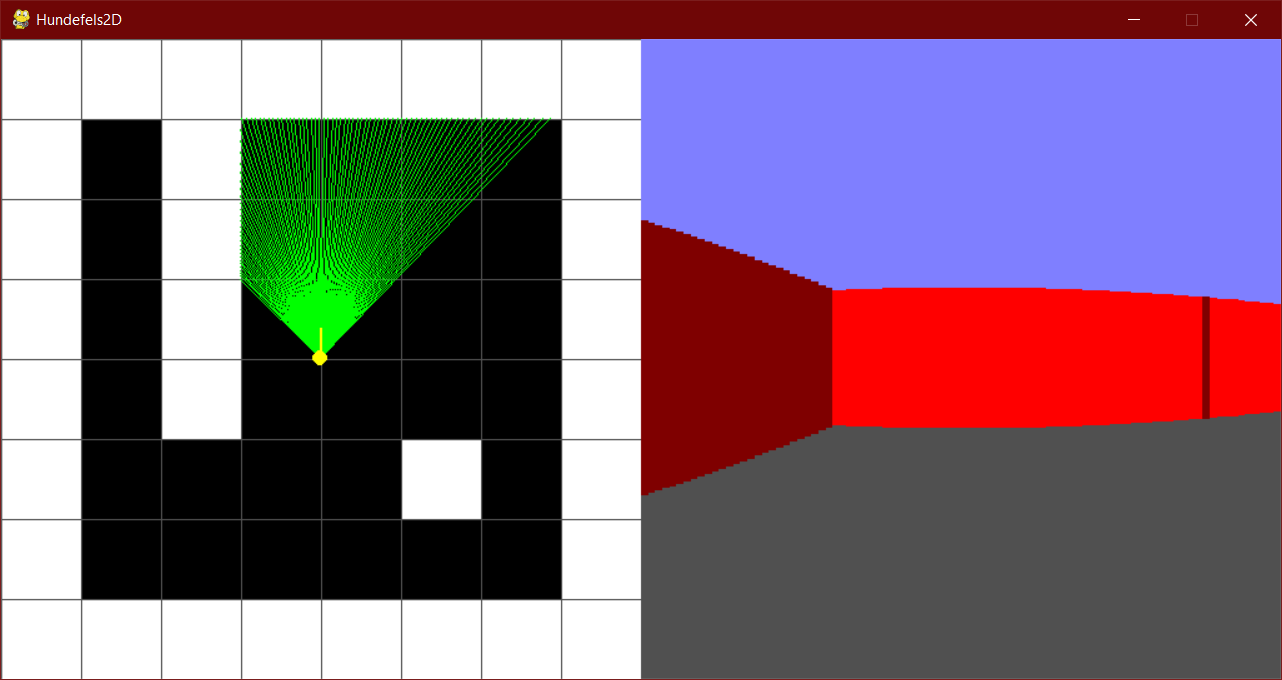
\includegraphics[scale=1.11]{./img/ui}\\
Das Anzeigefenster ist 1024 auf 512 Pixel groß.

Die linke Hälfte enthält die Kartenansicht. Der Spieler wird mit einem gelben Punkt darestellt, Entities mit (standartmässig) blauen Punkten.

Die rechte Hälfte des Fensters ist der First-Person Viewport.

\newpage

\begin{flushleft}
\begin{thebibliography}{99}
	
\bibitem{3dsage} 3DSage: ~ ``Make Your Own Raycaster Part 1'' ~ https://youtu.be/gYRrGTC7GtA\\ Quellcode verfügbar unter https://github.com/3DSage/OpenGL-Raycaster\_v1

\bibitem{pygametut} Pygame tutorial: 	https://www.pygame.org/docs/tut/MakeGames.html
\end{thebibliography}
\end{flushleft}

\end{document}